\section{Diagramme de cas d’utilisation global}
\subsection{Introduction}
\noindent
Dans cette partie, on va présenter les besoins de notre systéme de façon formelle à l'aide du diagramme de cas d'utilisation du langage de modélisation UML. D'abord nous identifions les acteurs qui intéragissent avec notre systéme, qui sont:

\noindent
\small\textbf{Le Visiteur: } C'est le personne qui va accéder à notre systéme pour rechercher le(s) produit(s) dans notre systéme.

\noindent
\small\textbf{Le Client: } C'est aussi le personne qui va accéder à notre systéme pour rechercher le(s) produit(s) de ses besoins. 

\noindent
\small\textbf{L'Admin: } C'est le personne qui va accéder à notre systéme pour rechercher le(s) produit(s) dans notre systéme et modifier les paramétres de son recherche. 

\begin{figure}[H]
\centering
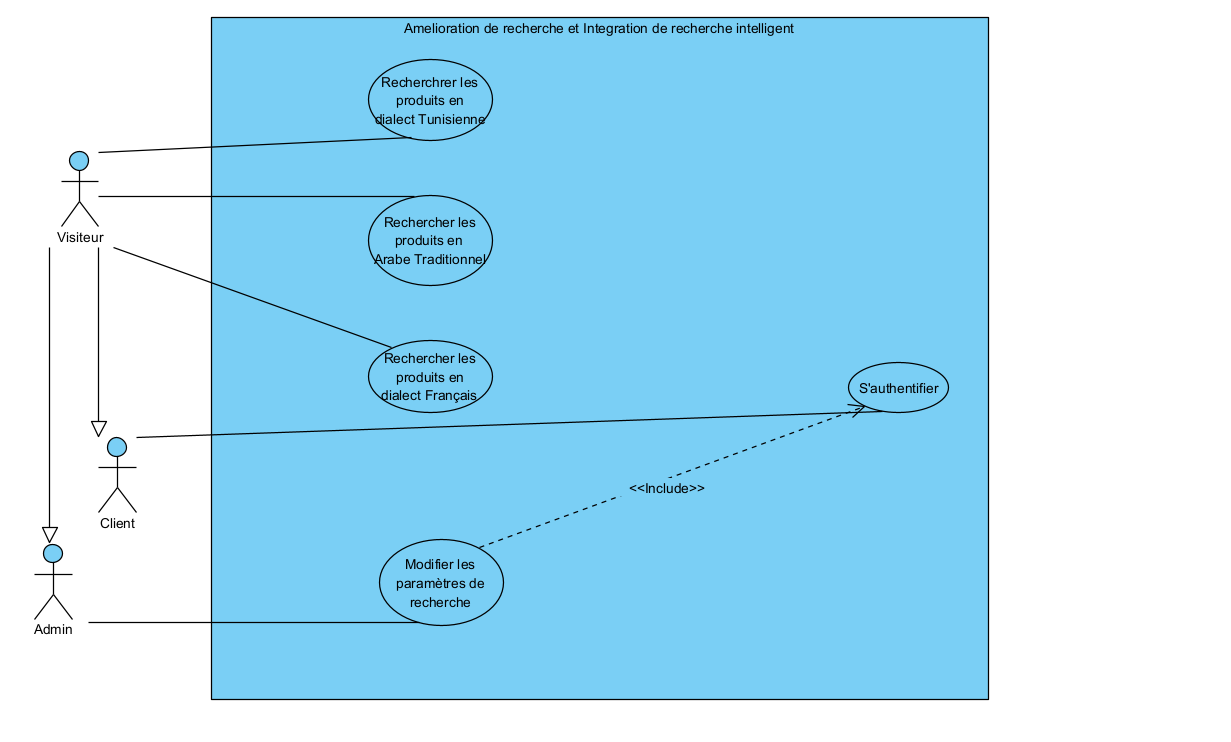
\includegraphics[width=1\textwidth]{logos/CU_global.png}
\caption{Présentation de Diagramme de Cas D'Utilisation global}
\label{fig:diagcuglobal}
\end{figure}